\begin{lstlisting}[float=p,label=lst:sdg-instances,
  caption={Program illustrating instances resulting in the SDG in \autoref{fig:sdg-instances}}]
class Main {
  static Main m1 = new Main();
  static Main m2 = new Main();
  
  int member;
  
  public static void main(String[] args) {
    int x = m1.foo(23);
    x += m1.foo(2) + m2.foo(3);
    System.out.println(x);
  }
  
  public int foo(int n) {
    member += n;
    return member;
  }
}
\end{lstlisting}

\begin{figure}[p]
  \centering
    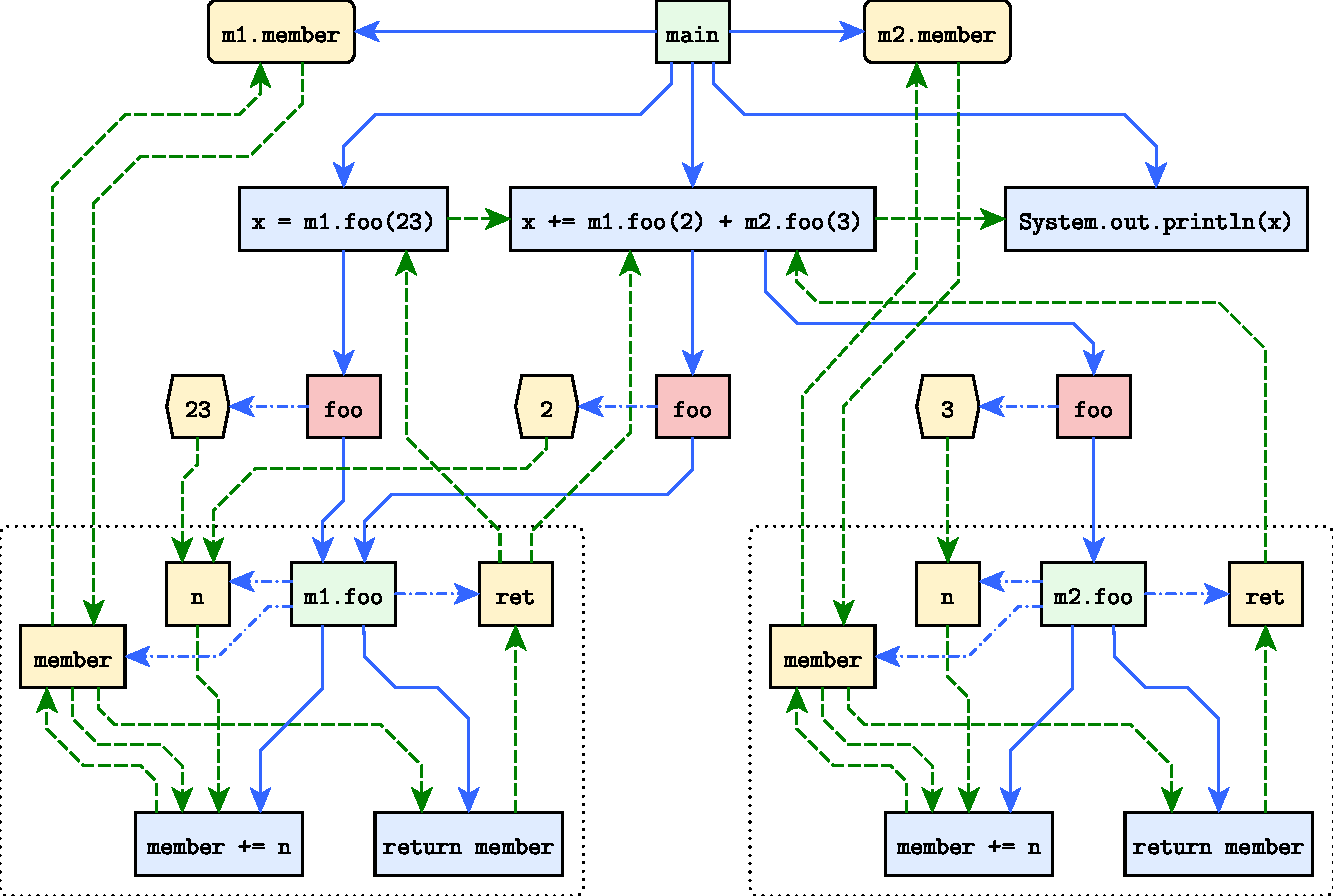
\includegraphics[scale=0.6]{sdgs/instances}
  \caption{SDG for the sample program in \autoref{lst:sdg-instances} (constructor calls omitted for brevity)}
  \label{fig:sdg-instances}
\end{figure}
